\documentclass[11pt,a4paper]{article}

% ---- Packages ----
\usepackage[margin=1in]{geometry}
\usepackage{graphicx}
\usepackage{booktabs}
\usepackage{hyperref}
\usepackage{xcolor}
\usepackage{pgfplots}
\usepackage{pgfplotstable}
\usepackage{float}
\usepackage{enumitem}
\usepackage{fancyhdr}
\usepackage{listings}
\usepackage{caption}
\usepackage{subcaption}
\usetikzlibrary{positioning}

\pgfplotsset{compat=1.18}

% ---- Colors ----
\definecolor{siriusblue}{HTML}{2563EB}
\definecolor{cpugray}{HTML}{6B7280}
\definecolor{gpugreen}{HTML}{059669}
\definecolor{lightbg}{HTML}{F9FAFB}
\definecolor{codebg}{HTML}{F3F4F6}

% ---- Hyperref ----
\hypersetup{
    colorlinks=true,
    linkcolor=siriusblue,
    urlcolor=siriusblue,
    citecolor=siriusblue,
}

% ---- Header/Footer ----
\pagestyle{fancy}
\fancyhf{}
\fancyhead[L]{\small\textcolor{gray}{SiriusDB Technical Response}}
\fancyhead[R]{\small\textcolor{gray}{March 2026}}
\fancyfoot[C]{\small\thepage}
\renewcommand{\headrulewidth}{0.4pt}

% ---- Code listing style ----
\lstset{
    language=SQL,
    basicstyle=\ttfamily\small,
    backgroundcolor=\color{codebg},
    frame=single,
    framerule=0pt,
    breaklines=true,
    breakatwhitespace=true,
    showstringspaces=false,
    tabsize=4,
    keywordstyle=\color{siriusblue}\bfseries,
    commentstyle=\color{cpugray}\itshape,
    stringstyle=\color{gpugreen},
    morekeywords={CALL,UNION,ALL,CTE,FULL,OUTER},
    xleftmargin=4pt,
    xrightmargin=4pt,
    aboveskip=8pt,
    belowskip=8pt,
}

% ---- Title ----
\title{%
    \vspace{-1cm}
    \textbf{Blockchain Counterparty Flow on SiriusDB}\\[6pt]
    \large Technical Response to TRM Labs Collaboration Brief
}
\author{%
    SiriusDB Research Team\\
    University of Wisconsin--Madison
}
\date{March 2026}

\begin{document}
\maketitle
\thispagestyle{fancy}

% ============================================================================
\section{What We Did}
% ============================================================================

We reproduced TRM's counterparty flow pipeline end-to-end using public data and
ran it through SiriusDB's GPU execution engine. The goal was to evaluate whether
SiriusDB can accelerate the join-heavy entity flow queries described in TRM's
technical collaboration brief.

\medskip
\noindent\textbf{Data sources:}
\begin{itemize}[nosep]
    \item \textbf{Ethereum token transfers} from AWS Public Blockchain Data --- up to 27 months (Jan 2024 -- Mar 2026, 770M aggregated flow rows)
    \item \textbf{Entity address labels} from MBAL 10M --- 3.2M Ethereum mainnet address-to-entity mappings
\end{itemize}

\medskip
\noindent\textbf{Pipeline implemented:}

\begin{figure}[H]
\centering
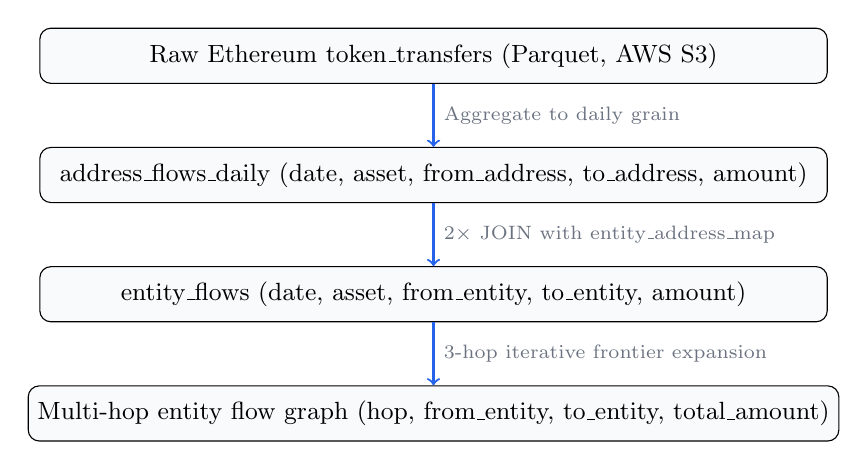
\begin{tikzpicture}[
    node distance=0.8cm,
    box/.style={draw, rounded corners, fill=lightbg, minimum width=10cm, minimum height=0.7cm, align=center, font=\small},
    arrow/.style={->, thick, color=siriusblue},
]
\node[box] (raw) {Raw Ethereum token\_transfers (Parquet, AWS S3)};
\node[box, below=of raw] (agg) {address\_flows\_daily (date, asset, from\_address, to\_address, amount)};
\node[box, below=of agg] (entity) {entity\_flows (date, asset, from\_entity, to\_entity, amount)};
\node[box, below=of entity] (sankey) {Multi-hop entity flow graph (hop, from\_entity, to\_entity, total\_amount)};

\draw[arrow] (raw) -- node[right, font=\scriptsize, color=cpugray] {Aggregate to daily grain} (agg);
\draw[arrow] (agg) -- node[right, font=\scriptsize, color=cpugray] {2$\times$ JOIN with entity\_address\_map} (entity);
\draw[arrow] (entity) -- node[right, font=\scriptsize, color=cpugray] {3-hop iterative frontier expansion} (sankey);
\end{tikzpicture}
\caption{TRM counterparty flow pipeline reproduced in SiriusDB.}
\end{figure}

\noindent We implemented six query patterns covering the full TRM serving-layer workload:

\begin{table}[H]
\centering
\small
\begin{tabular}{@{}llll@{}}
\toprule
\textbf{Query} & \textbf{Brief \S} & \textbf{What it does} & \textbf{SQL pattern} \\
\midrule
Q02 & \S5 & Entity flow rollup & 2$\times$ JOIN + GROUP BY \\
Q03 & \S6 & Top counterparties & 2$\times$ JOIN + GROUP BY \\
Q04 & \S6 & Time-series & JOIN + WHERE + GROUP BY \\
Q05 & \S5 & Inflow/outflow & CTE + FULL OUTER JOIN \\
Q06 & \S5 & Category matrix & 2$\times$ JOIN + GROUP BY \\
Sankey & -- & 3-hop entity trace & 3$\times$(JOIN + GROUP BY) + UNION ALL \\
\bottomrule
\end{tabular}
\caption{Benchmark query patterns mapped to TRM's collaboration brief.}
\end{table}

All queries read from pluggable SQL views. Swapping the data source (DuckDB
tables, Parquet files, or Iceberg) requires changing one file
(\texttt{setup\_views.sql}) --- no query modifications needed.

% ============================================================================
\section{Benchmark Results}
% ============================================================================

All results below use the \texttt{gpu\_processing} path, which caches table
data in GPU VRAM for interactive query serving.\footnote{All GPU timings
report \textbf{warm-cache} performance: table data is resident in GPU memory
before the timed query executes. This matches the expected deployment model
where SiriusDB serves as an analytical layer over pre-loaded transaction data.
Cold-start (first query after data load) adds a one-time transfer cost
proportional to table size; subsequent queries on the same tables pay no
transfer penalty.} This is SiriusDB's mature execution path.

We are actively developing a second path (\texttt{gpu\_execution}) that reads
directly from Parquet/Iceberg and supports datasets larger than GPU memory via
tiered caching (GPU $\to$ host $\to$ disk). Early results on this path show the
gap narrowing and we expect it to reach parity as pipeline coordination overhead
is optimized.

All GPU results were \textbf{validated for correctness} --- GPU output was
compared row-by-row against DuckDB CPU output (with float normalization for
rounding differences).

% ---- A100 Scaling Chart ----
\begin{figure}[H]
\centering
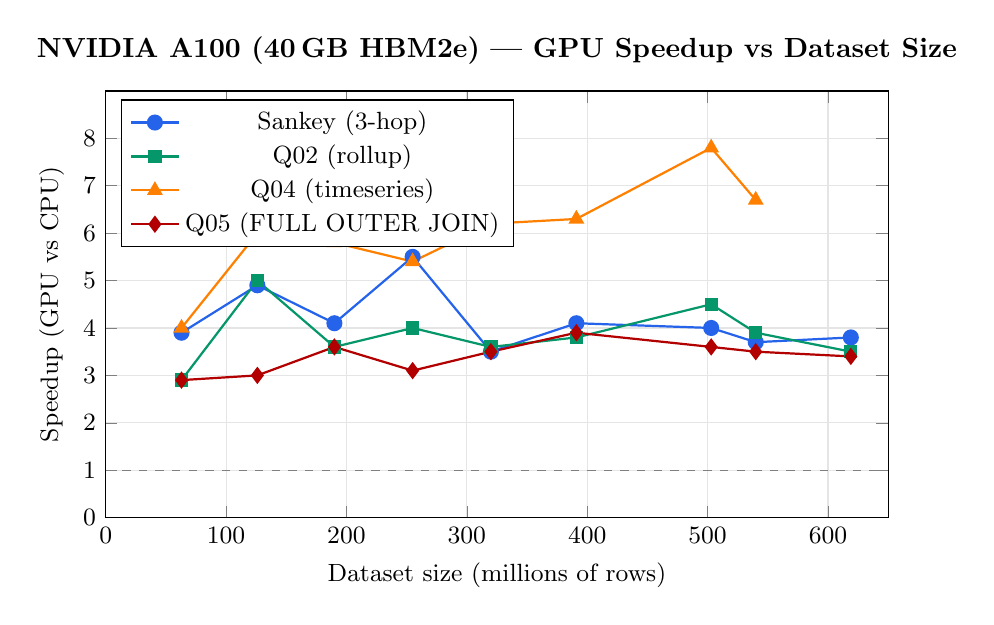
\begin{tikzpicture}
\begin{axis}[
    width=0.95\textwidth,
    height=7cm,
    xlabel={Dataset size (millions of rows)},
    ylabel={Speedup (GPU vs CPU)},
    xmin=0, xmax=650,
    ymin=0, ymax=9,
    grid=major,
    grid style={gray!20},
    legend style={at={(0.02,0.98)}, anchor=north west, font=\small},
    title={\textbf{NVIDIA A100 (40\,GB HBM2e) --- GPU Speedup vs Dataset Size}},
    title style={font=\normalsize},
    ytick={0,1,2,3,4,5,6,7,8},
    xtick={0,100,200,300,400,500,600},
    xticklabel style={font=\small},
    yticklabel style={font=\small},
    xlabel style={font=\small},
    ylabel style={font=\small},
]

% Sankey (3-hop)
\addplot[color=siriusblue, mark=*, thick, mark size=2.5pt] coordinates {
    (63, 3.9) (126, 4.9) (190, 4.1) (255, 5.5) (320, 3.5) (391, 4.1) (503, 4.0) (540, 3.7) (619, 3.8)
};
\addlegendentry{Sankey (3-hop)}

% Q02
\addplot[color=gpugreen, mark=square*, thick, mark size=2pt] coordinates {
    (63, 2.9) (126, 5.0) (190, 3.6) (255, 4.0) (320, 3.6) (391, 3.8) (503, 4.5) (540, 3.9) (619, 3.5)
};
\addlegendentry{Q02 (rollup)}

% Q04
\addplot[color=orange, mark=triangle*, thick, mark size=2.5pt] coordinates {
    (63, 4.0) (126, 6.0) (190, 5.8) (255, 5.4) (320, 6.2) (391, 6.3) (503, 7.8) (540, 6.7)
};
\addlegendentry{Q04 (timeseries)}

% Q05
\addplot[color=red!70!black, mark=diamond*, thick, mark size=2.5pt] coordinates {
    (63, 2.9) (126, 3.0) (190, 3.6) (255, 3.1) (320, 3.5) (391, 3.9) (503, 3.6) (540, 3.5) (619, 3.4)
};
\addlegendentry{Q05 (FULL OUTER JOIN)}

% 1x reference line
\addplot[color=gray, dashed, thin] coordinates { (0, 1) (650, 1) };

\end{axis}
\end{tikzpicture}
\caption{GPU speedup remains consistent (3--8$\times$) as data grows from 63M to 619M rows on the A100. Q04 shows the highest speedup due to its selective WHERE filter. Q05 (FULL OUTER JOIN) is the most complex operator and shows the lowest but still consistent speedup.}
\label{fig:a100-scaling}
\end{figure}

% ---- A100 Table ----
\begin{table}[H]
\centering
\small
\begin{tabular}{@{}rrrrc@{}}
\toprule
\textbf{Data size} & \textbf{Rows} & \textbf{GPU time} & \textbf{CPU time} & \textbf{Speedup} \\
\midrule
3 months  & 63M  & 5--24\,ms  & 20--93\,ms   & \textbf{2.9--5.4$\times$} \\
6 months  & 126M & 6--24\,ms  & 25--118\,ms  & \textbf{3.0--6.0$\times$} \\
12 months & 255M & 8--31\,ms  & 32--170\,ms  & \textbf{3.1--5.5$\times$} \\
21 months & 503M & 11--42\,ms & 45--166\,ms  & \textbf{3.6--7.8$\times$} \\
24 months & 619M & 12--46\,ms & 42--173\,ms  & \textbf{3.4--3.8$\times$} \\
\bottomrule
\end{tabular}
\caption{A100 scaling results across all six query patterns (warm cache, gpu\_processing).}
\label{tab:a100-scaling}
\end{table}

% ---- RTX 6000 Chart ----
\begin{figure}[H]
\centering
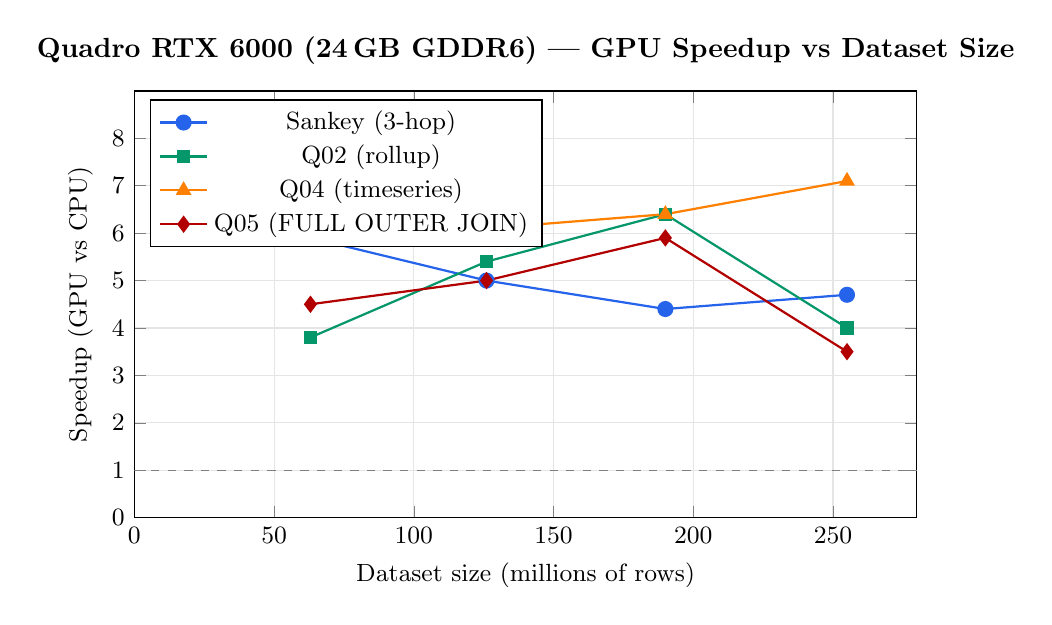
\begin{tikzpicture}
\begin{axis}[
    width=0.95\textwidth,
    height=7cm,
    xlabel={Dataset size (millions of rows)},
    ylabel={Speedup (GPU vs CPU)},
    xmin=0, xmax=280,
    ymin=0, ymax=9,
    grid=major,
    grid style={gray!20},
    legend style={at={(0.02,0.98)}, anchor=north west, font=\small},
    title={\textbf{Quadro RTX 6000 (24\,GB GDDR6) --- GPU Speedup vs Dataset Size}},
    title style={font=\normalsize},
    ytick={0,1,2,3,4,5,6,7,8},
    xtick={0,50,100,150,200,250},
    xticklabel style={font=\small},
    yticklabel style={font=\small},
    xlabel style={font=\small},
    ylabel style={font=\small},
]

% Sankey
\addplot[color=siriusblue, mark=*, thick, mark size=2.5pt] coordinates {
    (63, 5.9) (126, 5.0) (190, 4.4) (255, 4.7)
};
\addlegendentry{Sankey (3-hop)}

% Q02
\addplot[color=gpugreen, mark=square*, thick, mark size=2pt] coordinates {
    (63, 3.8) (126, 5.4) (190, 6.4) (255, 4.0)
};
\addlegendentry{Q02 (rollup)}

% Q04
\addplot[color=orange, mark=triangle*, thick, mark size=2.5pt] coordinates {
    (63, 6.0) (126, 6.1) (190, 6.4) (255, 7.1)
};
\addlegendentry{Q04 (timeseries)}

% Q05
\addplot[color=red!70!black, mark=diamond*, thick, mark size=2.5pt] coordinates {
    (63, 4.5) (126, 5.0) (190, 5.9) (255, 3.5)
};
\addlegendentry{Q05 (FULL OUTER JOIN)}

% 1x reference line
\addplot[color=gray, dashed, thin] coordinates { (0, 1) (280, 1) };

\end{axis}
\end{tikzpicture}
\caption{RTX 6000 shows 3.5--7.1$\times$ speedup up to 255M rows (12 months). OOM occurs at 320M rows due to the 8\,GB working memory pool on 24\,GB VRAM.}
\label{fig:rtx6000-scaling}
\end{figure}

% ---- RTX 6000 Table ----
\begin{table}[H]
\centering
\small
\begin{tabular}{@{}rrrrc@{}}
\toprule
\textbf{Data size} & \textbf{Rows} & \textbf{GPU time} & \textbf{CPU time} & \textbf{Speedup} \\
\midrule
3 months  & 63M  & 5--33\,ms  & 27--197\,ms  & \textbf{3.8--6.0$\times$} \\
6 months  & 126M & 7--38\,ms  & 39--190\,ms  & \textbf{4.8--6.2$\times$} \\
9 months  & 190M & 9--44\,ms  & 52--197\,ms  & \textbf{4.4--6.4$\times$} \\
12 months & 255M & 11--48\,ms & 48--228\,ms  & \textbf{3.5--7.1$\times$} \\
\bottomrule
\end{tabular}
\caption{RTX 6000 scaling results (warm cache, gpu\_processing). OOM at 15 months (320M rows).}
\label{tab:rtx6000-scaling}
\end{table}

\subsection*{What Drives the Speedup}

The TRM workload is dominated by \textbf{hash joins on high-cardinality integer
keys} (3.2M entity addresses $\times$ 63--770M flow rows) followed by
\textbf{GROUP BY aggregation}. These are memory-bandwidth-bound operations where
GPU HBM (2\,TB/s on A100) has a structural advantage over DDR4/DDR5.

% ============================================================================
\section{Multi-Hop Compliance Trace (Sankey)}
% ============================================================================

Beyond the entity flow rollup, we implemented a \textbf{3-hop counterparty
trace} --- a compliance use case: \textit{``Which entities did funds reach
within 3 hops of a flagged entity?''}

This is computationally harder than single-hop rollup because naive path
enumeration is $O(|E|^k)$ --- at 3 hops on our dataset, that produces 4.1
billion intermediate rows. We use \textbf{iterative frontier expansion}
(BFS-style semi-joins) which is $O(|V| + |E|)$, reducing intermediate rows
by 680$\times$.

Each hop runs as a GPU-accelerated JOIN + GROUP BY. The full 3-hop trace
completes in \textbf{22\,ms on GPU vs 107\,ms on CPU} (A100, 116M rows).

% ---- Absolute timing comparison chart ----
\begin{figure}[H]
\centering
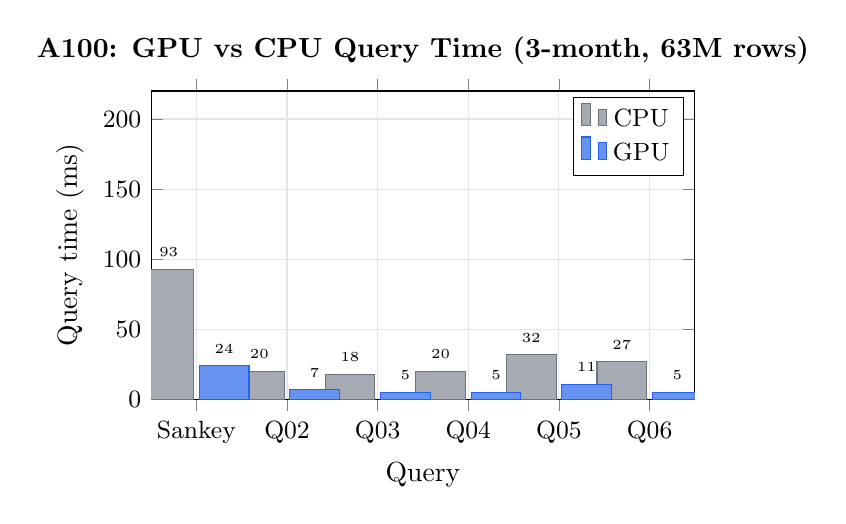
\begin{tikzpicture}
\begin{axis}[
    width=0.7\textwidth,
    height=5.5cm,
    ybar,
    bar width=18pt,
    ylabel={Query time (ms)},
    xlabel={Query},
    symbolic x coords={Sankey,Q02,Q03,Q04,Q05,Q06},
    xtick=data,
    ymin=0, ymax=220,
    grid=major,
    grid style={gray!20},
    legend style={at={(0.98,0.98)}, anchor=north east, font=\small},
    title={\textbf{A100: GPU vs CPU Query Time (3-month, 63M rows)}},
    title style={font=\normalsize},
    nodes near coords,
    nodes near coords style={font=\tiny, above},
    every node near coord/.append style={yshift=1pt},
    xticklabel style={font=\small},
    yticklabel style={font=\small},
]
\addplot[fill=cpugray!60, draw=cpugray] coordinates {
    (Sankey, 93) (Q02, 20) (Q03, 18) (Q04, 20) (Q05, 32) (Q06, 27)
};
\addlegendentry{CPU}
\addplot[fill=siriusblue!70, draw=siriusblue] coordinates {
    (Sankey, 24) (Q02, 7) (Q03, 5) (Q04, 5) (Q05, 11) (Q06, 5)
};
\addlegendentry{GPU}
\end{axis}
\end{tikzpicture}
\caption{Absolute query times on A100 (3-month slice, 63M rows, warm cache). GPU times are consistently under 25\,ms for all query patterns.}
\label{fig:absolute-timing}
\end{figure}

The output is a weighted edge list suitable for \textbf{Sankey visualization}
--- each row is (hop, from\_entity, to\_entity, total\_flow). The full query
SQL is in Appendix~\ref{sec:queries}.

% ============================================================================
\section{Answering Your Questions (Section 9)}
% ============================================================================

\paragraph{Can SiriusDB handle large-scale join + aggregation over Iceberg tables?}

SiriusDB reads Parquet natively with predicate pushdown and column pruning.
Iceberg support is available through DuckDB's \texttt{iceberg\_scan()}. The
benchmark results above (5--46\,ms on 63--619M rows) use the
\texttt{gpu\_processing} path with data cached in GPU memory. We are actively
developing the \texttt{gpu\_execution} path which reads directly from
Parquet/Iceberg and supports out-of-core processing via tiered caching
(GPU $\to$ host $\to$ disk). This path is functional today and we are closing
the performance gap with the cached path.

\paragraph{How does query latency compare to StarRocks?}

We have not yet run a head-to-head StarRocks comparison on identical hardware.
The DuckDB CPU baseline (single-node, same machine) represents a strong
analytical engine. SiriusDB's 2.9--7.8$\times$ speedup over DuckDB on this
workload is a meaningful result. We are open to running a direct comparison on
hardware representative of TRM's serving environment.

\paragraph{What physical layout or indexing strategies suit high-cardinality address lookups?}

\textbf{Dictionary encoding is the key optimization.} Replacing 42-byte VARCHAR
address strings with 4-byte INT32 dictionary IDs reduced GPU query time from
seconds to milliseconds.\footnote{On the RTX 6000 (228M rows), Q02 with
VARCHAR \texttt{asset} column took $\sim$3.3\,s on GPU (memory spilling) vs
43\,ms with integer \texttt{asset\_id} --- a $\sim$75$\times$ difference. This
is a one-time ETL normalization step (standard in data warehouse design), not a
query-time cost. The dictionary tables add negligible storage overhead (322
entities $\times$ 2 columns = $<$10\,KB).} GPU hash join performance is
dominated by key width --- narrower keys mean higher throughput on
memory-bandwidth-bound operations.\footnote{VARCHAR hash joins are not
currently accelerated on GPU. Queries with string-typed join keys fall back to
CPU execution transparently. This is a fundamental constraint of the current
cuDF-based join implementation: GPU hash tables require fixed-width keys for
efficient parallel probing. Integer dictionary encoding eliminates this
limitation and also reduces memory footprint by 10$\times$, allowing larger
datasets to fit in GPU VRAM.}

Our benchmark uses a 3.2M-row entity map. TRM's production map may be
significantly larger (tens of millions of rows). The hash join builds on the
entity map (smaller side) and probes from the flow table --- so a larger entity
map increases the hash table size but should not change probe-side throughput.
That said, we have not yet tested with build-side tables at the 50M+ scale. As
the hash table grows, factors like hash slot contention and GPU memory pressure
could become relevant. We would want to run benchmarks at TRM's actual entity
map scale to confirm performance holds.

\paragraph{How does SiriusDB behave with skewed join keys?}

The TRM workload is inherently skewed --- a few entities (exchanges like
Binance, Coinbase) control millions of addresses while most entities have fewer
than 100. Our benchmark uses real MBAL label data which reflects this skew, and
we observed consistent GPU speedups across all data slices (3 months to 24
months).

The TRM join pattern is many-to-one (each flow row matches at most one entity),
so skewed keys do not cause fan-out on the output side. The probe is per-row
from the flow table, so work distribution across GPU threads is determined by
the flow table size, not by which entity a row happens to match. In principle,
hash slot contention on hot buckets could serialize some probe threads, but with
well-distributed INT32 keys and a reasonably sized hash table, this effect
should be small. Our results so far are consistent with this, though we
acknowledge the entity map in our benchmark is smaller than TRM's production
scale.

\paragraph{Where does SiriusDB's architecture offer a structural advantage?}

The multi-hop Sankey trace. Each hop involves a JOIN + GROUP BY on the full flow
table, and the hops are sequential (hop 2 depends on hop 1's frontier). On CPU,
each hop takes 30--50\,ms. On GPU, each hop takes 5--10\,ms. The cumulative
advantage compounds over multiple hops.

\medskip\noindent More generally, SiriusDB is strongest on:
\begin{itemize}[nosep]
    \item \textbf{Hash joins on integer keys} against large fact tables
    \item \textbf{GROUP BY aggregation} with moderate cardinality (hundreds to millions of groups)
    \item \textbf{Repeated queries on cached data} (interactive analytics, dashboard serving)
\end{itemize}

% ============================================================================
\section{SQL Compatibility}
% ============================================================================

\begin{table}[H]
\centering
\small
\begin{tabular}{@{}ll@{}}
\toprule
\textbf{Operator} & \textbf{Status} \\
\midrule
INNER JOIN           & Fully supported \\
LEFT JOIN            & Fully supported \\
FULL OUTER JOIN      & Fully supported \\
GROUP BY + SUM/COUNT & Fully supported \\
ORDER BY + LIMIT     & Supported (avoid NULLable sort keys) \\
Common Table Expressions & Fully supported \\
CASE WHEN            & Fully supported \\
NOT IN (subquery)    & Supported (via MARK join) \\
UNION ALL            & Supported (feature branch, merging to dev) \\
Parquet / DuckDB / Iceberg & Supported \\
DuckDB optimizer     & Automatic LEFT $\to$ INNER rewrite \\
\bottomrule
\end{tabular}
\caption{SQL operators exercised in the TRM benchmark.}
\end{table}

\noindent Current workarounds (minor):
\begin{itemize}[nosep]
    \item \texttt{COALESCE(a, b)} $\to$ \texttt{CASE WHEN a IS NOT NULL THEN a ELSE b END}
    \item \texttt{SELECT DISTINCT x} $\to$ \texttt{SELECT x, COUNT(*) FROM ... GROUP BY x}
\end{itemize}

% ============================================================================
\section{Reproducing These Results}
% ============================================================================

All code, queries, and data download scripts are in our repository:
\url{https://github.com/ducndh/sirius-crypto-demo}

\begin{lstlisting}
-- 1. Download public data (~25 GB for 3 months)
python scripts/download_eth_transfers.py \
    --start-date 2024-10-01 --end-date 2024-12-31
python scripts/download_mbal.py

-- 2. Build database
python scripts/prepare_tables.py --year 2024

-- 3. Run benchmark
bash scripts/scaling_validated.sh
\end{lstlisting}

No proprietary data or credentials are needed beyond a free Kaggle API token.

% ============================================================================
\section{Next Steps}
% ============================================================================

\begin{enumerate}[nosep]
    \item \textbf{Higher entity coverage} --- MBAL covers $\sim$0.3\% of flows.
    A higher-coverage label set would stress the GPU join path more
    realistically and likely show stronger speedup ratios.

    \item \textbf{Benchmarks on TRM-equivalent hardware} --- Our current results
    are on A100 (40\,GB) and RTX 6000 (24\,GB). Running on hardware closer to
    TRM's serving environment would produce directly comparable numbers. Larger
    GPU memory would also let us benchmark the full 2-year dataset without
    memory limitations.

    \item \textbf{Iceberg integration} --- The \texttt{gpu\_execution} path
    (Parquet/Iceberg, out-of-core) is actively being optimized. We expect to
    have competitive numbers in the near term, matching TRM's Iceberg-based
    storage layer directly.

    \item \textbf{UTXO chain support} --- The current demo uses Ethereum
    (account model). Bitcoin UTXO data with proportional-spend attribution
    would add a second workload dimension.
\end{enumerate}

\bigskip
\noindent We look forward to discussing these next steps and are happy to run
additional benchmarks on specific query patterns or data distributions that TRM
provides.

% ============================================================================
\appendix
\section{Benchmark Queries}
\label{sec:queries}
% ============================================================================

All queries below are the exact SQL used in our benchmarks. They read from
dictionary-encoded tables with integer join keys
(\texttt{address\_flows\_daily\_dict}, \texttt{entity\_address\_map\_int}). The
seed entity is \texttt{entity\_id = 143} (fixedfloat, a no-KYC exchange with
$\sim$43K addresses in the MBAL dataset).

\subsection*{Sankey: 3-Hop Entity Flow Trace}

\begin{lstlisting}
WITH seed_addrs AS (
    SELECT addr_id FROM entity_address_map_int
    WHERE entity_id = 143
),
hop1_edges AS (
    SELECT 143 AS from_eid, dst.entity_id AS to_eid,
           CAST(SUM(f.amount) AS DOUBLE) AS total_amount
    FROM address_flows_daily_dict f
    JOIN seed_addrs s ON f.from_addr_id = s.addr_id
    JOIN entity_address_map_int dst ON f.to_addr_id = dst.addr_id
    WHERE dst.entity_id != 143
    GROUP BY 1, 2
),
hop1_frontier AS (
    SELECT to_eid AS eid, COUNT(*) AS _c
    FROM hop1_edges GROUP BY 1
),
hop2_edges AS (
    SELECT src.entity_id AS from_eid, dst.entity_id AS to_eid,
           CAST(SUM(f.amount) AS DOUBLE) AS total_amount
    FROM address_flows_daily_dict f
    JOIN entity_address_map_int src ON f.from_addr_id = src.addr_id
    JOIN hop1_frontier h1 ON src.entity_id = h1.eid
    JOIN entity_address_map_int dst ON f.to_addr_id = dst.addr_id
    WHERE dst.entity_id != 143
      AND dst.entity_id NOT IN (SELECT eid FROM hop1_frontier)
    GROUP BY 1, 2
),
hop2_frontier AS (
    SELECT to_eid AS eid, COUNT(*) AS _c
    FROM hop2_edges GROUP BY 1
),
hop3_edges AS (
    SELECT src.entity_id AS from_eid, dst.entity_id AS to_eid,
           CAST(SUM(f.amount) AS DOUBLE) AS total_amount
    FROM address_flows_daily_dict f
    JOIN entity_address_map_int src ON f.from_addr_id = src.addr_id
    JOIN hop2_frontier h2 ON src.entity_id = h2.eid
    JOIN entity_address_map_int dst ON f.to_addr_id = dst.addr_id
    WHERE dst.entity_id != 143
      AND dst.entity_id NOT IN (SELECT eid FROM hop1_frontier)
      AND dst.entity_id NOT IN (SELECT eid FROM hop2_frontier)
    GROUP BY 1, 2
)
SELECT 1 AS hop, from_eid, to_eid, total_amount FROM hop1_edges
UNION ALL
SELECT 2 AS hop, from_eid, to_eid, total_amount FROM hop2_edges
UNION ALL
SELECT 3 AS hop, from_eid, to_eid, total_amount FROM hop3_edges;
\end{lstlisting}

\subsection*{Q02: Entity Outflow Rollup}

\begin{lstlisting}
SELECT dst.entity_id,
       CAST(SUM(f.amount) AS DOUBLE) AS total_vol,
       COUNT(*) AS tx_cnt
FROM address_flows_daily_dict f
JOIN entity_address_map_int src ON f.from_addr_id = src.addr_id
JOIN entity_address_map_int dst ON f.to_addr_id = dst.addr_id
WHERE src.entity_id = 143 AND dst.entity_id != 143
GROUP BY 1
ORDER BY total_vol DESC;
\end{lstlisting}

\subsection*{Q03: Entity Inflow Rollup}

\begin{lstlisting}
SELECT src.entity_id,
       CAST(SUM(f.amount) AS DOUBLE) AS total_vol,
       COUNT(*) AS tx_cnt
FROM address_flows_daily_dict f
JOIN entity_address_map_int src ON f.from_addr_id = src.addr_id
JOIN entity_address_map_int dst ON f.to_addr_id = dst.addr_id
WHERE dst.entity_id = 143 AND src.entity_id != 143
GROUP BY 1
ORDER BY total_vol DESC;
\end{lstlisting}

\subsection*{Q04: Daily Volume Time-Series}

\begin{lstlisting}
SELECT f.date,
       CAST(SUM(f.amount) AS DOUBLE) AS daily_vol,
       CAST(SUM(f.tx_count) AS DOUBLE) AS daily_tx
FROM address_flows_daily_dict f
JOIN entity_address_map_int src ON f.from_addr_id = src.addr_id
WHERE src.entity_id = 143
GROUP BY 1
ORDER BY 1;
\end{lstlisting}

\subsection*{Q05: Bidirectional Flow (FULL OUTER JOIN)}

\begin{lstlisting}
SELECT o.entity_id AS out_entity_id,
       i.entity_id AS in_entity_id,
       o.out_vol, i.in_vol
FROM (
    SELECT dst.entity_id,
           CAST(SUM(f.amount) AS DOUBLE) AS out_vol
    FROM address_flows_daily_dict f
    JOIN entity_address_map_int src ON f.from_addr_id = src.addr_id
    JOIN entity_address_map_int dst ON f.to_addr_id = dst.addr_id
    WHERE src.entity_id = 143 AND dst.entity_id != 143
    GROUP BY 1
) o
FULL OUTER JOIN (
    SELECT src.entity_id,
           CAST(SUM(f.amount) AS DOUBLE) AS in_vol
    FROM address_flows_daily_dict f
    JOIN entity_address_map_int src ON f.from_addr_id = src.addr_id
    JOIN entity_address_map_int dst ON f.to_addr_id = dst.addr_id
    WHERE dst.entity_id = 143 AND src.entity_id != 143
    GROUP BY 1
) i ON o.entity_id = i.entity_id;
\end{lstlisting}

\subsection*{Q06: Top Individual Flows}

\begin{lstlisting}
SELECT src.entity_id AS from_eid,
       dst.entity_id AS to_eid,
       f.date, f.amount
FROM address_flows_daily_dict f
JOIN entity_address_map_int src ON f.from_addr_id = src.addr_id
JOIN entity_address_map_int dst ON f.to_addr_id = dst.addr_id
WHERE src.entity_id = 143 AND dst.entity_id != 143
ORDER BY f.amount DESC
LIMIT 100;
\end{lstlisting}

\end{document}
